
\documentclass[letterpaper,11pt]{article}
\usepackage[utf8]{inputenc}
\usepackage[spanish]{babel}
\usepackage{mathtools}
\usepackage{graphicx}

\begin{document}

\title{Estructura de datos\\\large Actividad 7}
\author{Dagoberto Quevedo}
\maketitle

\begin{abstract}
En esta actividad se realiza en primera instancia la diferencia conceptual y abstracta entre arreglos y listas, posteriormente se realiza la implementación computacional de un algoritmo clásico de recuento de inversas con una variante de implementación usando arreglos y en otra listas.
\end{abstract}

\section{Arreglos y listas}

\subsection{Arreglos}

Un arreglo es una colección ordena de elementos, donde cada uno de ellos dentro del arreglo tiene un índice. Los índices de los elementos pueden iniciar desde cero $a[]=[a_0,\dots,a_{n-1}]$ o alternativamente uno $a[]=[a_1,\dots,a_{n}]$. El tiempo de acceso a un elemento con índice $k$ es $\mathcal{O}(1)$, el tiempo para determinar si un elemento $x$ exista en $a$ es $\mathcal{O}(n)$, se asume que los elementos guardados no están ordenados.

\subsection{Listas}

Las listas son una colección de elementos (también llamados nodos) ordenados de manera secuencial y enlazados con un puntero con el elemento siguiente. Agregar un nuevo elemento o nodo es en tiempo $\mathcal{O}(1)$, por lo general las listas se implementan como listas enlazadas (individual, doble, circular, etc.) o cómo matriz dinámica (redimensionables). Para insertar un nuevo elemento $v$ después de $u$, se ajusta el puntero de $v$ para que apunte ahora a $u$. La operación de eliminación es similar, si se elimina el elemento $v$ que precede a $u$, entonces el puntero del elemento que precede a $v$, que puede ser $q$ apuntará a $u$.

\begin{figure}[h!]
  \centering
  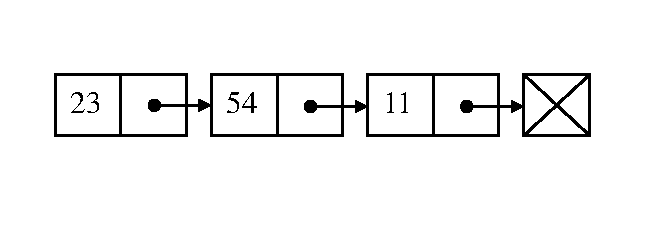
\includegraphics[width=8cm]{img/img_list.pdf}
  \caption{Representación gráfica de una lista enlazada. La primer celda del nodo expresa el dato y la segunda el puntero que enlaza al siguiente nodo.}
  \label{fig:ie}
\end{figure}



\subsection{Diferencias entre ambas estructuras}

La principal diferencia entre las dos estructuras de datos es un acceso secuencial o acceso directo. Los arreglos permiten ambos accesos, mientras que las listas solo acceso secuenciales. Si bien con las listas se logra flexibilidad y escalabilidad en el tamaño dinámico de las estructuras, las búsquedas y consultas de un elemento tienen un costo de $\mathcal{O}(n)$ a diferencia de los arreglos que tiene un costo de acceso de $\mathcal{O}(1)$.


\section{Implementación computacional}

Se realiza la implementación computacional del algoritmo recuento de inversas, el cual se define como dado un vector $A$, encontrar el número de inversas posibles de este, si $(i <j)$ y $a_i > a_j$ entonces el par ordenado $(i,j)$ es llamado como una inversa del vector $A$. Se realizan dos implementaciones de este método:

\begin{itemize}
	\item \textit{Ingenuo}: Es la solución simple debido a que por cada elemento del vector se cuenta todos los elementos menores que su derecha que cumplan la condición $a_i > a_j$. La complejidad de esta solución es $\mathcal{O}(n^2)$. Se realiza la implementación a través de arreglos.
	\item \textit{Ordenamiento por mezcla}: Este problema  puede resolverse usando un ordenamiento de mezcla. Básicamente para cada elemento del vector, contamos todos los elementos mayores que a su izquierda. Esta implementación permite el uso de listas y recursividad. La complejidad de esta solución es $\mathcal{O}(n\log n)$.
\end{itemize}


\subsection{Condiciones de experimentación}
Se realiza la implementación computacional en Python, la evaluación se realiza ejecutando una serie de instancias, en este caso cada instancia se define como un vector $A$ de tamaño ${2^n}$ con elementos enteros seleccionados aleatoriamente con una distribución uniforme en un rango $[1,1\times 10^8]$, donde $n\in \{1,\dots,15\}$, la ejecución se repite $k=10$ veces.

\subsection{Resultados}
El gráfico \ref{fig:bs} muestra los resultados del diseño experimental en el tiempo de computo expresado en escala logarítmica, el eje vertical expresa el valor de $n$ que define el tamaño de la instancia ${2^n}$. 

\begin{figure}[h]
 \centering
  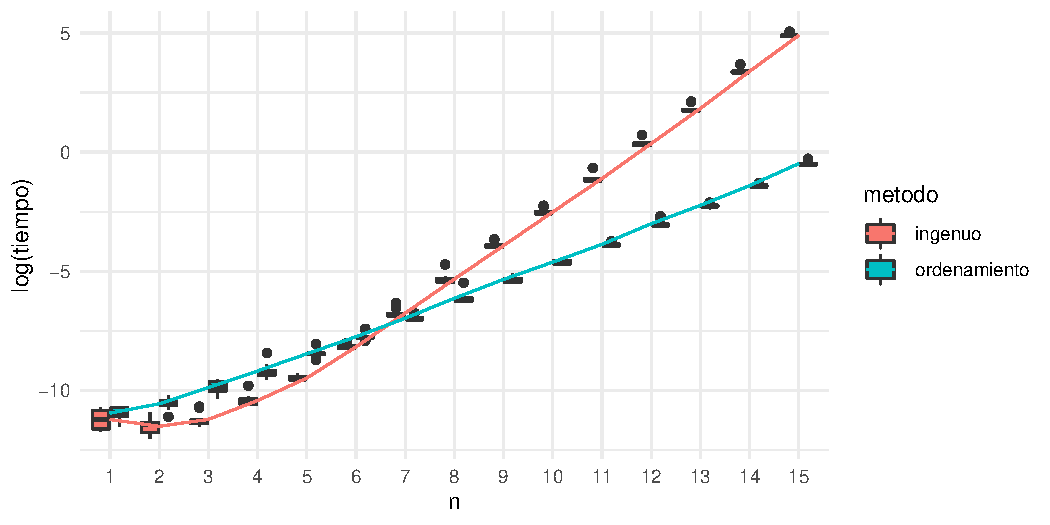
\includegraphics[width=11.5cm]{img/A7.pdf}
  \caption{Resultados del diseño experimental con $k=10$ ejecuciones para cada tipo de implementación.}
  \label{fig:bs}
\end{figure}

\subsection{Conclusiones}

Basado en el resultado gráfico del experimento, el ordenamiento por mezclas es superior en función del tiempo requerido para converge a un resultado, esto se anticipa dado la complejidad de este método es menor a la requerida por el método básico o ingenuo. Si bien este experimento no se logra captar el aporte de cada una de las estructuras, si se puede discernir que la implementación ingenua sólo es posible a través de arreglos y el ordenamiento por mezclas permite mayor flexibilidad en el uso de arreglos o listas.


\begin{thebibliography}{0}
  \bibitem{Knuth1998} Donald Knuth, \textit{Sorting and searching}, The Art of Computer Programming, Addison-Wesley Professional, 1998.
  \bibitem{Schaeffer2020} Elisa Schaeffer, \textit{Modelos computacionales}, Complejidad computacional de problemas y el análisis y diseño de algoritmos, notas de curso, 2020.
\end{thebibliography}


\end{document}
